\documentclass[openany,12pt]{memoir}
\usepackage[utf8]{inputenc} 
\usepackage[czech]{babel}
\usepackage[T1]{fontenc}
\usepackage[top=1.5cm, bottom=2cm, left=2cm, right=2cm]{geometry}  % --> NASTAVENÍ OKRAJŮ
\usepackage{fancyhdr}
\usepackage{graphicx}
%\usepackage{xwatermark}
\usepackage{xcolor}
\usepackage{changepage}
\usepackage{pdfpages}
\usepackage{lettrine}
\usepackage{indentfirst}  %Důležité pro formátování
\usepackage[pages=some]{background}

%%%%%%%%%%%%%%%%%%%%%%%%%%%%%%%%%%%%%%
%  FONT                              %
%%%%%%%%%%%%%%%%%%%%%%%%%%%%%%%%%%%%%%
\usepackage{amssymb}
\usepackage{tgschola}

%%%%%%%%%%%%%%%%%%%%%%%%%%%%%%%%%%%%%%
%  Obrázky v textu                   %
%%%%%%%%%%%%%%%%%%%%%%%%%%%%%%%%%%%%%%
\usepackage{tikz}
%\tikz[remember picture,overlay] \node[opacity=0.3,inner sep=0pt] at (current page.center){\includegraphics[width=\paperwidth,height=\paperheight]{example-image}};
%Tímto příkazem se na následující stránku vloží pozadí. Pokud pozadí uděláme
%tak, aby bylo velikosti a4, bylo prázdné až na malůvku, můžeme takto vkládat
%obrázky.
%Pozn.: kompilovat se musí dvakrát


%%%%%% Package na zpěvník
\usepackage[full]{leadsheets}%http://mirrors.nic.cz/tex-archive/macros/latex/contrib/leadsheets/leadsheets_en.pdf   --> dokumentace	
\definesongtitletemplate{empty}{} 
\setchords{
format = \bfseries \sffamily,   %tučné akordy
minor = {mi},% 
input-notation = {german},%
output-notation = {german}%
}
\definesongtitletemplate{empty}{} 


\newlength{\drop}
% VODOZNAK
%\newwatermark[pages=1-,color=red!50,angle=0,scale=2, xpos=0,ypos=0]{\includegraphics[width=5cm]{obr/pozadi2.jpg}} %--> dvojka na pozadí


%%%%%%%%%%%%%%%%%%%%%%%%%%%%%%%%%%%%%%%%%%%%%%%%%%
%		 Vlastní příkazy
\newcommand{\defaulttabscale}{0.87}
\newcommand{\defaultfretscale}{1.7}

\newcounter{Slokočet}   %Automatické číslování slok
\newcommand{\mezera}{
\phantom{.}

}   %Horizontální odsazení slok (poněkud blbě zadefinovaný, ale jinak se formát rozbije jako wtf prostě)
\newcommand{\stred}{5.2cm}   %%% Na zarovnání slok doprostřed, pozn. automatičtější zarovnávání na střed nejde
\newcommand{\carka}{,\:}
\newcommand{\m}[1]{\color{white}{#1}}  %Pro akordy
\newcommand{\ap}{'}	%Pro apostrof
\newcommand{\elipsa}{\kern\fontdimen3\font} %Příkaz pro lepší zacházení s výpustkami (=...); je to vpodstatě jen mezera mezi tečkama výpustky
\newcommand{\pindent}{17.62482 pt} %Správná velikost \parindentu u layoutu se dvěma minipageama
\newcommand{\predtitle}{\huge}
\newcommand{\mezisloupci}{\phantom{TT}} %Místo mezi dvěma sloupci na jedné stránce
\newcommand{\z}{\hspace*{\fill}\null}

%%% Možné velikosti písem 
\newcommand{\normalni}{\normalsize}
\newcommand{\velky}{\fontsize{14.4}{15}\selectfont}
\newcommand{\vetsi}{\fontsize{15}{16}\selectfont}
\newcommand{\nejvetsi}{\fontsize{16}{17}\selectfont}
\newcommand{\nejnejvetsi}{\fontsize{17}{19}\selectfont}

%%% Stará definice sloky spoléhající na indenty
%\newlength{\pismeno}
%\settowidth{\pismeno}{x} %Tohle není moc ideální velikost, ale funguje
%\newif\ifslokavelka
%\slokavelkafalse
%\newcommand{\sloka}{
%\ifnum \value{Slokočet}>8  %Pokud je sloka dvouciferná
%\mezera \noindent \addtocounter{Slokočet}{1} \hspace*{-\pismeno}\arabic{Slokočet}.
%\else %Pokud jen jednociferná
%\mezera \noindent \addtocounter{Slokočet}{1} \arabic{Slokočet}. 
%\fi
%} 	%sloka, která se automaticky čísluje

\newcommand{\distanc}{\:}  %Vzdálenost čísla sloky před slokou
\newlength{\delkaargumentu}
%%% Sloka s automatickým číslováním
\newcommand{\sloka}{%
\addtocounter{Slokočet}{1}% Zvýší se o 1 počet slok
\mezera%  Sloka se odsadí vertikálně
\settowidth{\delkaargumentu}{\arabic{Slokočet}.\distanc}% Zde se určí délka odsazení 
\hspace*{-\delkaargumentu}%
\arabic{Slokočet}.\distanc%
\ignorespaces% Aby nevznikaly zbytečné mezery
}


%%% Sloka s vlastním argumentem
\newcommand{\ssloka}[1]{%     
\settowidth{\delkaargumentu}{#1\distanc}
\mezera%
\hspace*{-\delkaargumentu}%
#1\distanc%
\ignorespaces%
}  

%%% Refrén
\newcommand{\refren}[1][0]{%  Nepovinný argument sděluje, kolikátý refrén toto je, bez argumentu se vytiskne pouze refrén
\ifnum #1>0 %Pokud nepovinný argument existuje
\mezera%
\settowidth{\delkaargumentu}{\textbf{R$_{\text{#1}}$:}\distanc}%
\hspace*{-\delkaargumentu}%
\textbf{R$_{\text{#1}}$:}\distanc%
\ignorespaces%
\else %Pokud nepovinný argument neexistuje
\mezera%
\settowidth{\delkaargumentu}{\textbf{R:}\distanc}%
\hspace*{-\delkaargumentu}%
\textbf{R:}\distanc%
\ignorespaces%
\fi
}

\newcommand{\predehra}{\ssloka{\textbf{Předehra:}}}

%%% Capo
\newcommand{\kapodastr}[1]{%
\textit{Capo {#1}}
}

\newcommand{\includefret}[1]{\includegraphics[scale=\defaultfretscale]{../Akordy/msc/#1.pdf}}

\addto\captionsczech{\renewcommand{\contentsname}{Seznam písní}}

%%%%%%%%%%%%%%%%%%%%%%%%%%%%%%%%%%%%
%    FORMÁTOVÁNÍ                   %
%%%%%%%%%%%%%%%%%%%%%%%%%%%%%%%%%%%%

%%% Vlevo zarovnaný text s blokem zarovnaným na střed
\usepackage{varwidth}% http://ctan.org/pkg/varwidth
\newenvironment{centerjustified}{%
  \begin{center} % so the minipage is centered
  \begin{varwidth}[t]{\textwidth}	
  \raggedright % so the minipage's text is left justified
  \setlength{\parindent}{\pindent}
}{%
  \end{varwidth}
  \end{center}
}

%%% Pozadí
\newcommand{\pozadi}[1]{
\backgroundsetup{
scale=1,
angle=0,
contents={%
  \includegraphics[width=\paperwidth,height=\paperheight]{#1}
  }%
}
\BgThispage
}


%Hlavnička END
\usepackage{hyperref}
\begin{document}
\sffamily %Sans-serif pro lepší čitelnost

\pagestyle{empty}
\newgeometry{top=1.5cm, bottom = 0cm, left = 2cm, right = 2cm}

\newpage

%Pro kompilaci je důležitý, aby ten \input a \end{document} zůstali na posledních
%dvou řádcích!!!!

\velky
\newpage
% PÍSNIČKA

\begin{song}{title=\predtitle \centering John Brown's Body \\\large  }  %% sem se napíše jméno songu a autor


\vspace*{-0.43cm}
\vetsi

\moveleft 0.6cm \vbox{

\begin{centerjustified}
\begin{varwidth}[t]{0.5\textwidth}\setlength{\parindent}{\pindent}  %Varianta č. 2 --> Dva sloupce

\vspace*{-0.43cm}


\sloka
^{G\z}John Brown’s body lies moldering in

the grave,

While ^{C\z}weep the sons of bondage whom

he ^{G\z}ventured all to save;

But tho he lost his life while struggling

for the ^{Emi}slave,

His ^{A7}soul is ^{D7\z}marching ^{G}on.

\refren
^{G\z}Glory, glory, hallelujah!

^{C\z}Glory, glory, ^{G}hallelujah!

Glory, glory, ^{\z Emi}hallelujah!

^{Ami\z }his~soul's ^{D7\z}marching ^{G}on!

\sloka
John Brown was a hero, undaunted,

true and brave,

And Kansas knows his valor when he

fought her rights to save;

Now, tho the grass grows green above

his grave,

His soul is marching on.

\refren

\sloka
He captured Harper’s Ferry, with his

nineteen men so few,

And frightened Old Virginny till she

trembled thru and thru;

They hung him for a traitor,

themselves the traitor crew,

But his soul is marching on.

\refren



\end{varwidth}\begin{varwidth}[t]{0.55\textwidth}\setlength{\parindent}{\pindent}
\vspace*{0.03cm}


\sloka
John Brown was John the Baptist of the

Christ we are to see,

Christ who of the bondmen shall the

Liberator be,

And soon throug the Sunny South the

slaves shall all be free,

For his soul is marching on.

\refren


\sloka
The conflict that he heralded he looks from

heaven to view,

On the army of the Union with its flag red,

white and blue.

And heaven shall ring with anthems o’er

the deed they mean to do,

For his soul is marching on.

\refren

\sloka
Ye soldiers of Freedom, then strike, while

strike ye may,

The death blow of oppression in a better

time and way,

For the dawn of old John Brown has

brightened into day,

And his soul is marching on.

\refren

\hrulefill

\vspace*{.1cm}

\begin{varwidth}{.5\textwidth}
Otroctví bylo v USA zakázáno r. 1865.

I~dnes otroctví v~jistých částech světa přetrvává.
%např. firma
%Nestlé prý používá dětské otroky.

Afroameričané však stále v~USA čelí systémovému rasismu.
Např. v~r. 2022 je v~tamních vězeních celkem 2 miliony lidí, z toho 38 \% Afr.,
i~když tvoří jen 12 \% populace.
\end{varwidth}
\begin{varwidth}{.2\textwidth}
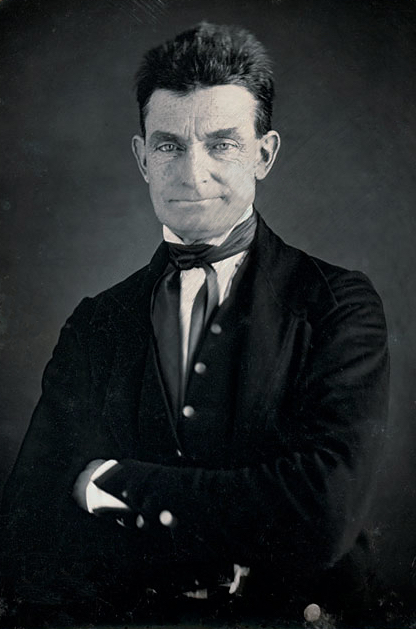
\includegraphics[width=4cm]{../img/JohnBrown.jpg}
\end{varwidth}



\end{varwidth}
\end{centerjustified}


}




\setcounter{Slokočet}{0}
\end{song}


\end{document}
